Via \href{https://zeppelin.flights/@dmoren/}{@dmoren@zeppelin.flights}:
\url{https://zeppelin.flights/@dmoren/112400352858244906} \#retoot

\begin{figure}
\centering
\pandocbounded{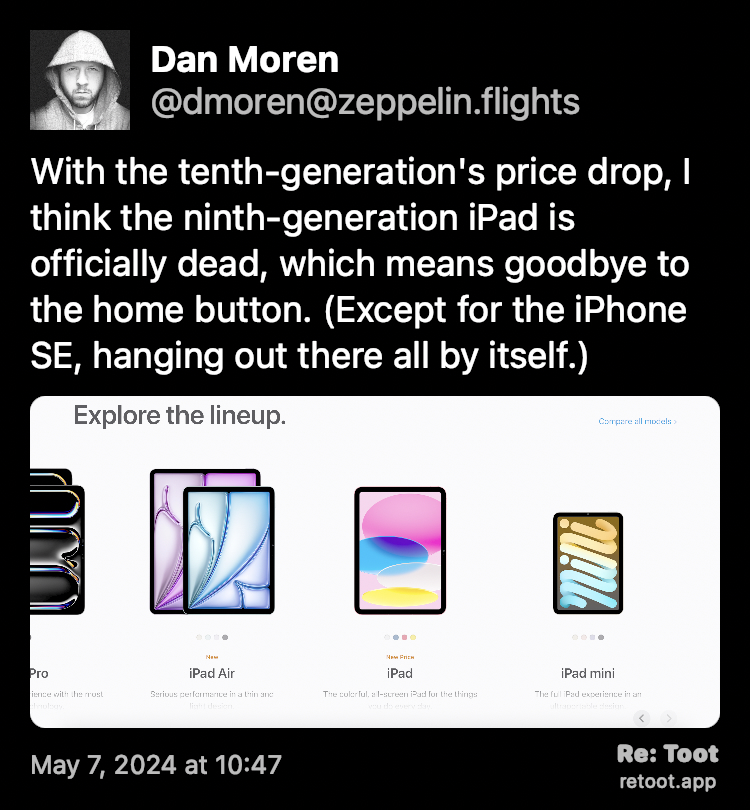
\includegraphics[keepaspectratio]{\%7B\%7Bsite.url\%7D\%7D/img/moren-pad.jpg}}
\caption{Post by Dan Moren. ``With the tenth-generation's price drop, I
think the ninth-generation iPad is officially dead, which means goodbye
to the home button. (Except for the iPhone SE, hanging out there all by
itself.)'' The post contains an image with the following description:
``Screenshot from Apple.com showing iPad Pro, iPad Air, iPad, and iPad
mini.'' Posted on May 7, 2024 at 10:47}
\end{figure}

\begin{quote}
\emph{Post by Dan Moren. ``With the tenth-generation's price drop, I
think the ninth-generation iPad is officially dead, which means goodbye
to the home button. (Except for the iPhone SE, hanging out there all by
itself.)'' The post contains an image with the following description:
``Screenshot from Apple.com showing iPad Pro, iPad Air, iPad, and iPad
mini.'' Posted on May 7, 2024 at 10:47}
\end{quote}

Is it bad that I really want a home button simply for manual dexterity
issues? This feels like an accessibility concern.

Via
\href{https://mastodon.social/@macrumors/}{@macrumors@mastodon.social}:
\url{https://mastodon.social/@macrumors/112400357673551779} \#retoot

\begin{figure}
\centering
\pandocbounded{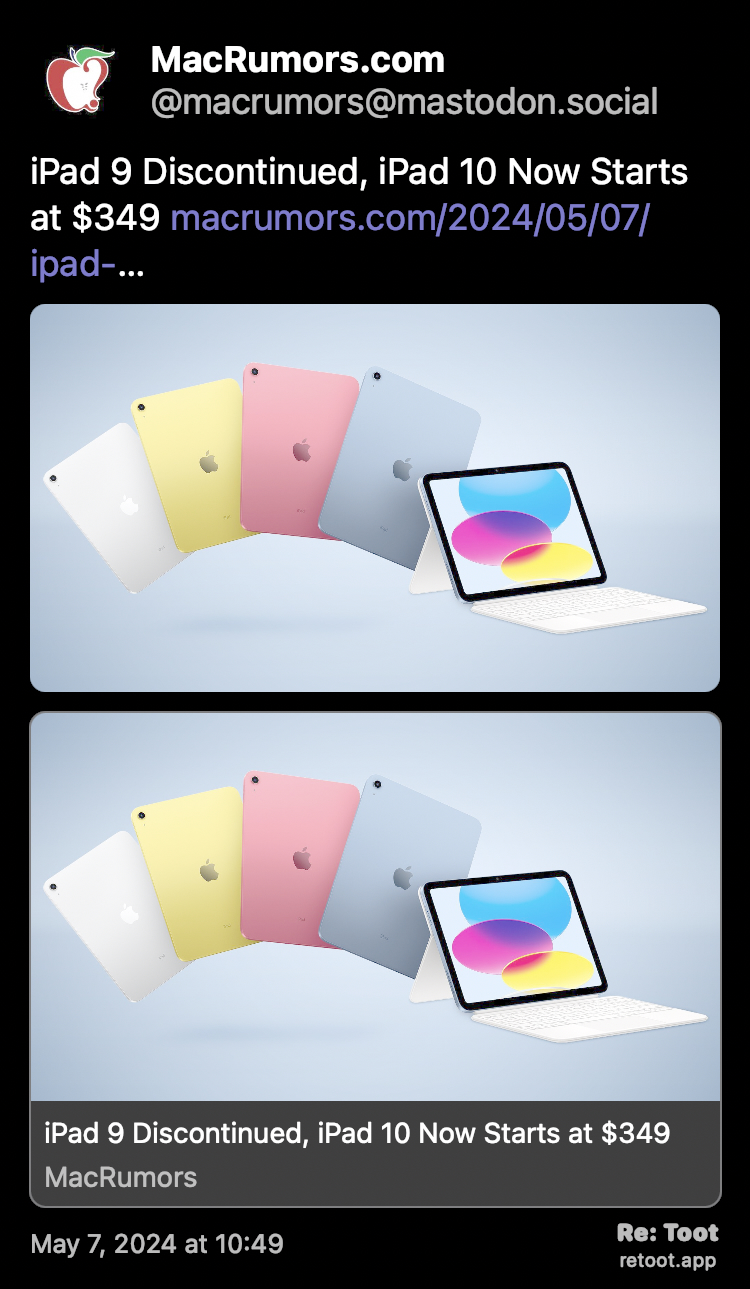
\includegraphics[keepaspectratio]{\%7B\%7Bsite.url\%7D\%7D/img/double-discontinued.jpg}}
\caption{Post by MacRumors.com. ``iPad 9 Discontinued, iPad 10 Now
Starts at \$349 macrumors.com/2024/05/07/ipad-\ldots{}'' The post
contains an image with no description. Posted on May 7, 2024 at 10:49}
\end{figure}

\begin{quote}
\emph{Post by MacRumors.com. ``iPad 9 Discontinued, iPad 10 Now Starts
at \$349 macrumors.com/2024/05/07/ipad-\ldots{}'' The post contains an
image with no description. Posted on May 7, 2024 at 10:49}
\end{quote}

My current iPad is now double discontinued. That is to say,
\href{https://www.macrumors.com/2024/05/07/ipad-9-discontinued-ipad-10-now-starts-at-349/}{the
generation after my current iPad just got discontinued}. I suppose I
\emph{may} be due for an upgrade soon enough.

Lots to think about in this situation, I suppose.

And finally\ldots{}

Via \href{https://wandering.shop/@aleen/}{@aleen@wandering.shop}:
\url{https://wandering.shop/@aleen/112400227162075413} \#retoot

\begin{figure}
\centering
\pandocbounded{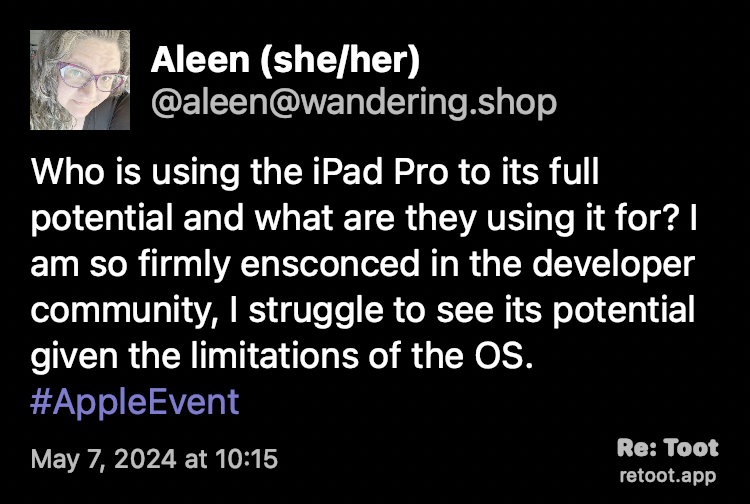
\includegraphics[keepaspectratio]{\%7B\%7Bsite.url\%7D\%7D/img/seeking-use-case.jpg}}
\caption{Post by Aleen (she/her). ``Who is using the iPad Pro to its
full potential and what are they using it for? I am so firmly ensconced
in the developer community, I struggle to see its potential given the
limitations of the OS. \#AppleEvent'' Posted on May 7, 2024 at 10:15}
\end{figure}

\begin{quote}
\emph{Post by Aleen (she/her). ``Who is using the iPad Pro to its full
potential and what are they using it for? I am so firmly ensconced in
the developer community, I struggle to see its potential given the
limitations of the OS. \#AppleEvent'' Posted on May 7, 2024 at 10:15}
\end{quote}

Convertible sub-Macbook. That's the only use case I can \emph{currently}
think of. Something else might arise, I suppose.
